
\newcommand{\topx}{\ensuremath{X~}}
\newcommand{\catTop}{\textsf{Top}}

\begin{frame}
    \frametitle{Exercise 3.4 - 15}
    \textit{Problem Statement}\\
    Let \topx be a \emph{finite} topological space. Show that the following are
    equivalent:
    \begin{enumerate}
        \item \topx has the discrete topology.
        \item \topx is metrizable.
        \item \topx is Hausdorff.
    \end{enumerate}
\end{frame}

\begin{frame}
    \frametitle{Establishing Relationships}
    \centering
    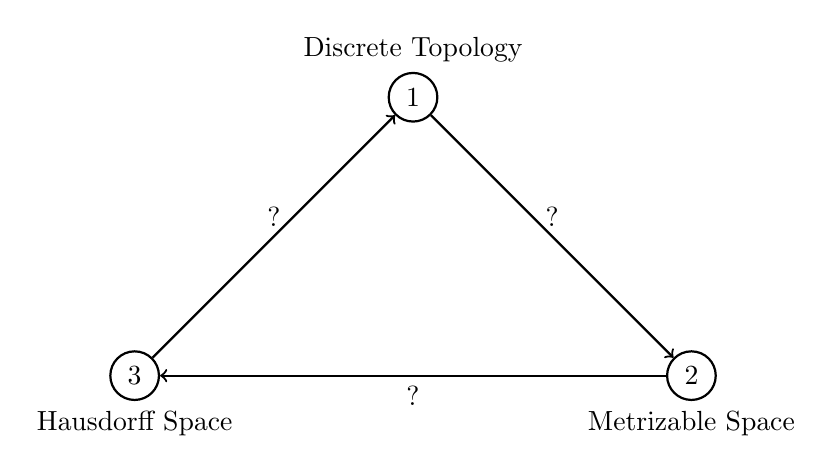
\begin{tikzpicture}[node distance={5cm}, thick, main/.style = {draw, circle}]
        \node[main, label=above:Discrete Topology] (1)                      {\(1\)};
        \node[main, label=below:Metrizable Space] (2) [below right of=1]    {\(2\)};
        \node[main, label=below:Hausdorff Space] (3) [below left of=1]      {\(3\)};

        % \pause

        \draw[->] (1) -- node[midway, above] {?} (2);
        \draw[->] (2) -- node[midway, below] {?} (3);
        \draw[->] (3) -- node[midway, above] {?} (1);

    \end{tikzpicture}

\end{frame}

\begin{frame}
    \frametitle{\(1 \rightarrow 2\) --- Discrete \(\rightarrow\) Metrizable}

    % discrete space
    show discrete space

    \pause

    % map to real line
    real line

\end{frame}

\begin{frame}
    \frametitle{\(2 \rightarrow 3\) --- Metrizable \(\rightarrow\) Hausdorff}

    % metrizable, existence of metric
    metric

    % construct ball and shrink
    ball

\end{frame}

\begin{frame}
    \frametitle{\(3 \rightarrow 1\) --- Hausdorff \(\rightarrow\) Discrete}

    % construct Hausdorff sets
    Hausdorff

    % show point exclusion
    exclusion

    % intersect
    intersect

\end{frame}

\begin{frame}
    \frametitle{Establishing Relationships}
    \centering
    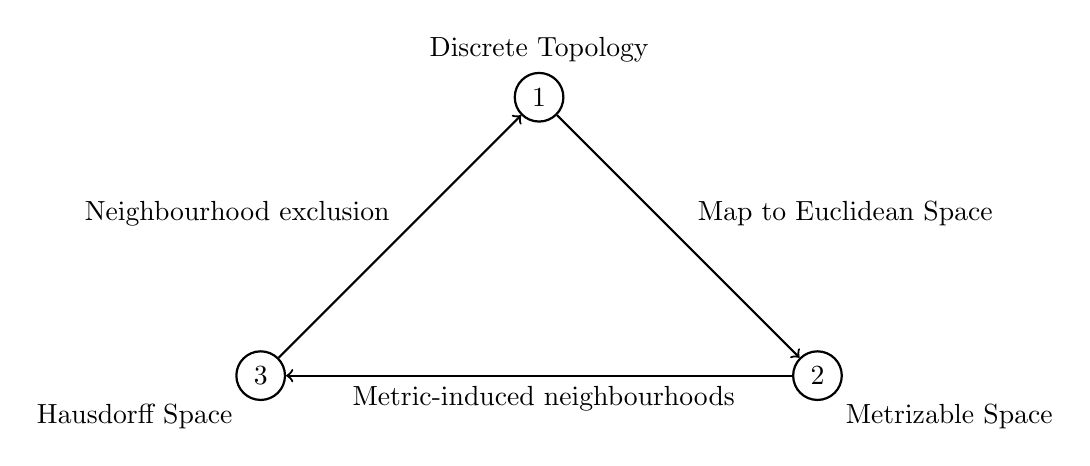
\begin{tikzpicture}[node distance={5cm}, thick, main/.style = {draw, circle}]
        \node[main, label=above:Discrete Topology] (1)                      {\(1\)};
        \node[main, label=below right:Metrizable Space] (2) [below right of=1]    {\(2\)};
        \node[main, label=below left:Hausdorff Space] (3) [below left of=1]      {\(3\)};

        % \pause

        \draw[->] (1) -- node[midway, above right] {\(\checkmark\) Map to Euclidean Space} (2);
        \draw[->] (2) -- node[midway, below] {\(\checkmark\) Metric-induced neighbourhoods} (3);
        \draw[->] (3) -- node[midway, above left] {\(\checkmark\) Neighbourhood exclusion} (1);

    \end{tikzpicture}

\end{frame}